\documentclass[12pt]{article}
\usepackage[margin=1.5cm]{geometry}
\usepackage{parskip}
\usepackage{amsmath}
\usepackage{amssymb}
\usepackage{amsfonts}
\usepackage{enumitem}
\usepackage{graphicx}
\usepackage{stmaryrd}
\graphicspath{ {./images/} }


\begin{document}
\begin{enumerate}[label=(\alph*)]
  \item
    \begin{enumerate}[label=(\roman*)]
      \item
        There are a few problems that would cause rapid route change, or route flapping.

        For example, if a link is broken in such a way that it repeatedly comes online and offline, then the (likely link-state) routing information will rapidly change, and routes could oscillate based on whether or not this link is detected as online or not. In protocols like BGP, if this happens internally in an AS, then the AS will keep advertising different routes and information, causing large oscillations in the route state.

        We might also face issues with route loops in distance-vector protocols. For example in the topology below, when the link BC fails, A and B will loop distance-vector messages, continuously updating their routes.

        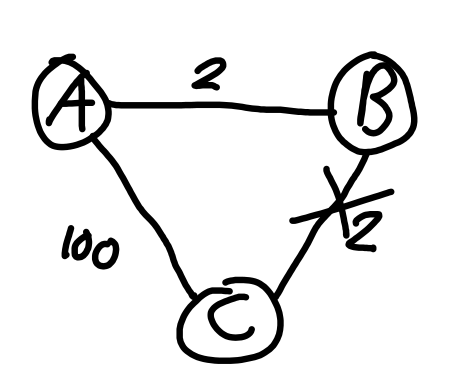
\includegraphics[scale=0.3]{loop}

      \item
        A feedback control system can be used to damp these oscillations by essentially punishing routers for sending too many routing updates, essentially hysteresis. If they change a route too much, then they are rate limited, and this penalty decays exponentially over time, but may increase again if the issues are still occurring.
        
    \end{enumerate}

  \item
    A controller could operate to adjust TCP's congestion control by measuring the rate of packets for a particular flow, and adjusting this to the congestion window of the flow with ECN marked packets. We assume here that we manage the queue explicitly, i.e. we might purposely drop the packets to force the flow to a particular flow rate (similar to RED).

    The benefit of a PID controller over AIMD is that we achieve a stable flow rate over time, instead of sawtooth-like behaviour. This means that the behaviour isn't to overshoot, and then punish, instead just staying at the accurate rate, meaning that hopefully we get less congestion and less packet loss.

    This is mostly non-examinable.



        
\end{enumerate}
\end{document}
